\documentclass[twoside, 10pt]{article}

\usepackage{geometry}
\geometry{bottom=4em,top=6em, inner=2.2cm, outer=4em,  headheight=\paperheight}
\usepackage[export]{adjustbox}
\usepackage{array}
\usepackage{amsmath}
\usepackage{amsfonts}
\usepackage{fancyhdr}
\pagestyle{fancy}
\fancyhf{}
\lhead{Precalculus - BASE}
\chead{Review of Slope}
\rhead{Practice, Page \thepage}
\usepackage{lastpage}
\usepackage{xcolor}
\usepackage{enumitem}
\usepackage{pifont}
\usepackage{graphicx}
\graphicspath{{../img}}
\usepackage{pgfplots}
\pgfplotsset{compat=1.18}
\usepackage{tabularx}

\newcommand{\R}{\mathbb R}
\newcommand{\e}{{\rm e}}
\newcommand{\pobr}[1]{\left\langle#1\right\rangle}
\newcommand{\norm}[1]{\lVert #1 \rVert}
\newcommand{\abs}[1]{\lvert #1 \rvert}

\DeclareMathOperator{\xd}{d\!}
\DeclareMathOperator{\proj}{proj}

\title{}
\date{}

\begin{document}
\noindent
{\large
First Name \rule{6em}{.1pt}\hspace{\stretch{1}}Last Name \rule{6em}{.1pt}\hspace{\stretch{1}} Date \rule{1.5em}{.1pt} -- \rule{1.5em}{.1pt} -- \rule{1.5em}{.1pt}\hspace{\stretch{1}} Period \rule{2em}{.1pt}\hspace{\stretch{1}} Score \rule{2em}{.1pt}
}
\vspace{1em}
Let $A$ be $(1,2)$ and $B$ be $(2,4)$. 
\begin{enumerate}
\item Plot $A$ and $B$ on the coordinate axes below (label them), then sketch the line containing them.

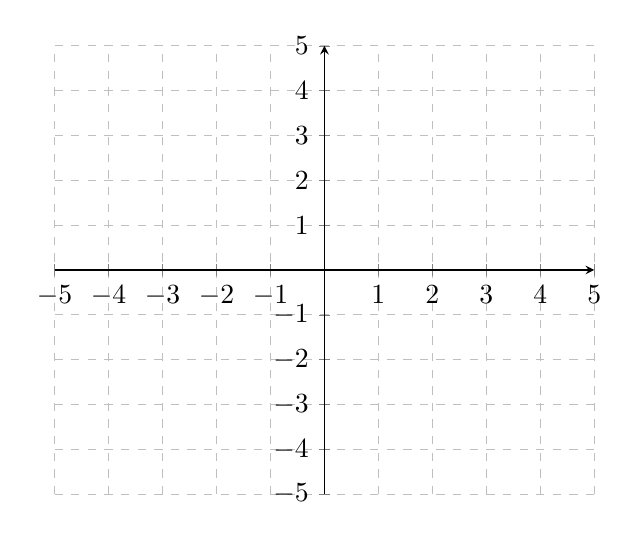
\begin{tikzpicture}
\begin{axis}[
axis lines = middle,
ymax=5, ymin=-5,
xmax=5, xmin=-5,
xtick distance = 1,
ytick distance=1,
grid style={dashed},
grid=both
]
\end{axis}
\end{tikzpicture}
\item Find the slope of the line $AB$, then find an equation of $AB$.
\vspace{\stretch{1}}
\item Determine if $(3,5)$ is a point on $AB$.
\vspace{\stretch{1}}
\item Find the equation of the line parallel to $AB$ and containing the point $(6,7)$.
\vspace{\stretch{1}}
\end{enumerate}

\end{document}